\section{Explanation maps}

Figure~\ref{fig:maps} shows, for one test image of melanoma, basal cell carcinoma and nevus, which regions each fine-tuned model's prediction is sensitive to.
For ResNet-50 I use Grad-CAM~\cite{selvaraju2017gradcam} on the last convolutional block; for ViT-Base I use attention rollout~\cite{abnar2020quantifying}, which multiplies the head-averaged attention matrices of all layers (with the residual connection added) and reads off the attention from the class token to each patch.
Both maps are computed for the class the model predicts; they are produced by \texttt{scripts/visualize.py}.

These maps are qualitative.
The images are simply the first test image of each of the three classes, not chosen for how the maps look.
In all three, the ResNet-50 Grad-CAM map lies mostly on the lesion.
The ViT attention-rollout maps are more diffuse and also give high values to image corners and borders, including the ruler marks in the bottom-right corner of the melanoma image.
Three images cannot show whether this means ViT relies on such artefacts or is a property of attention rollout itself.
ViT misclassifies the basal cell carcinoma as melanoma with low confidence (0.29), whereas ResNet-50 classifies it correctly.
None of this demonstrates that either model relies on clinically meaningful features.

\begin{figure}[h]
\centering
\IfFileExists{supplementary/attention_map.png}{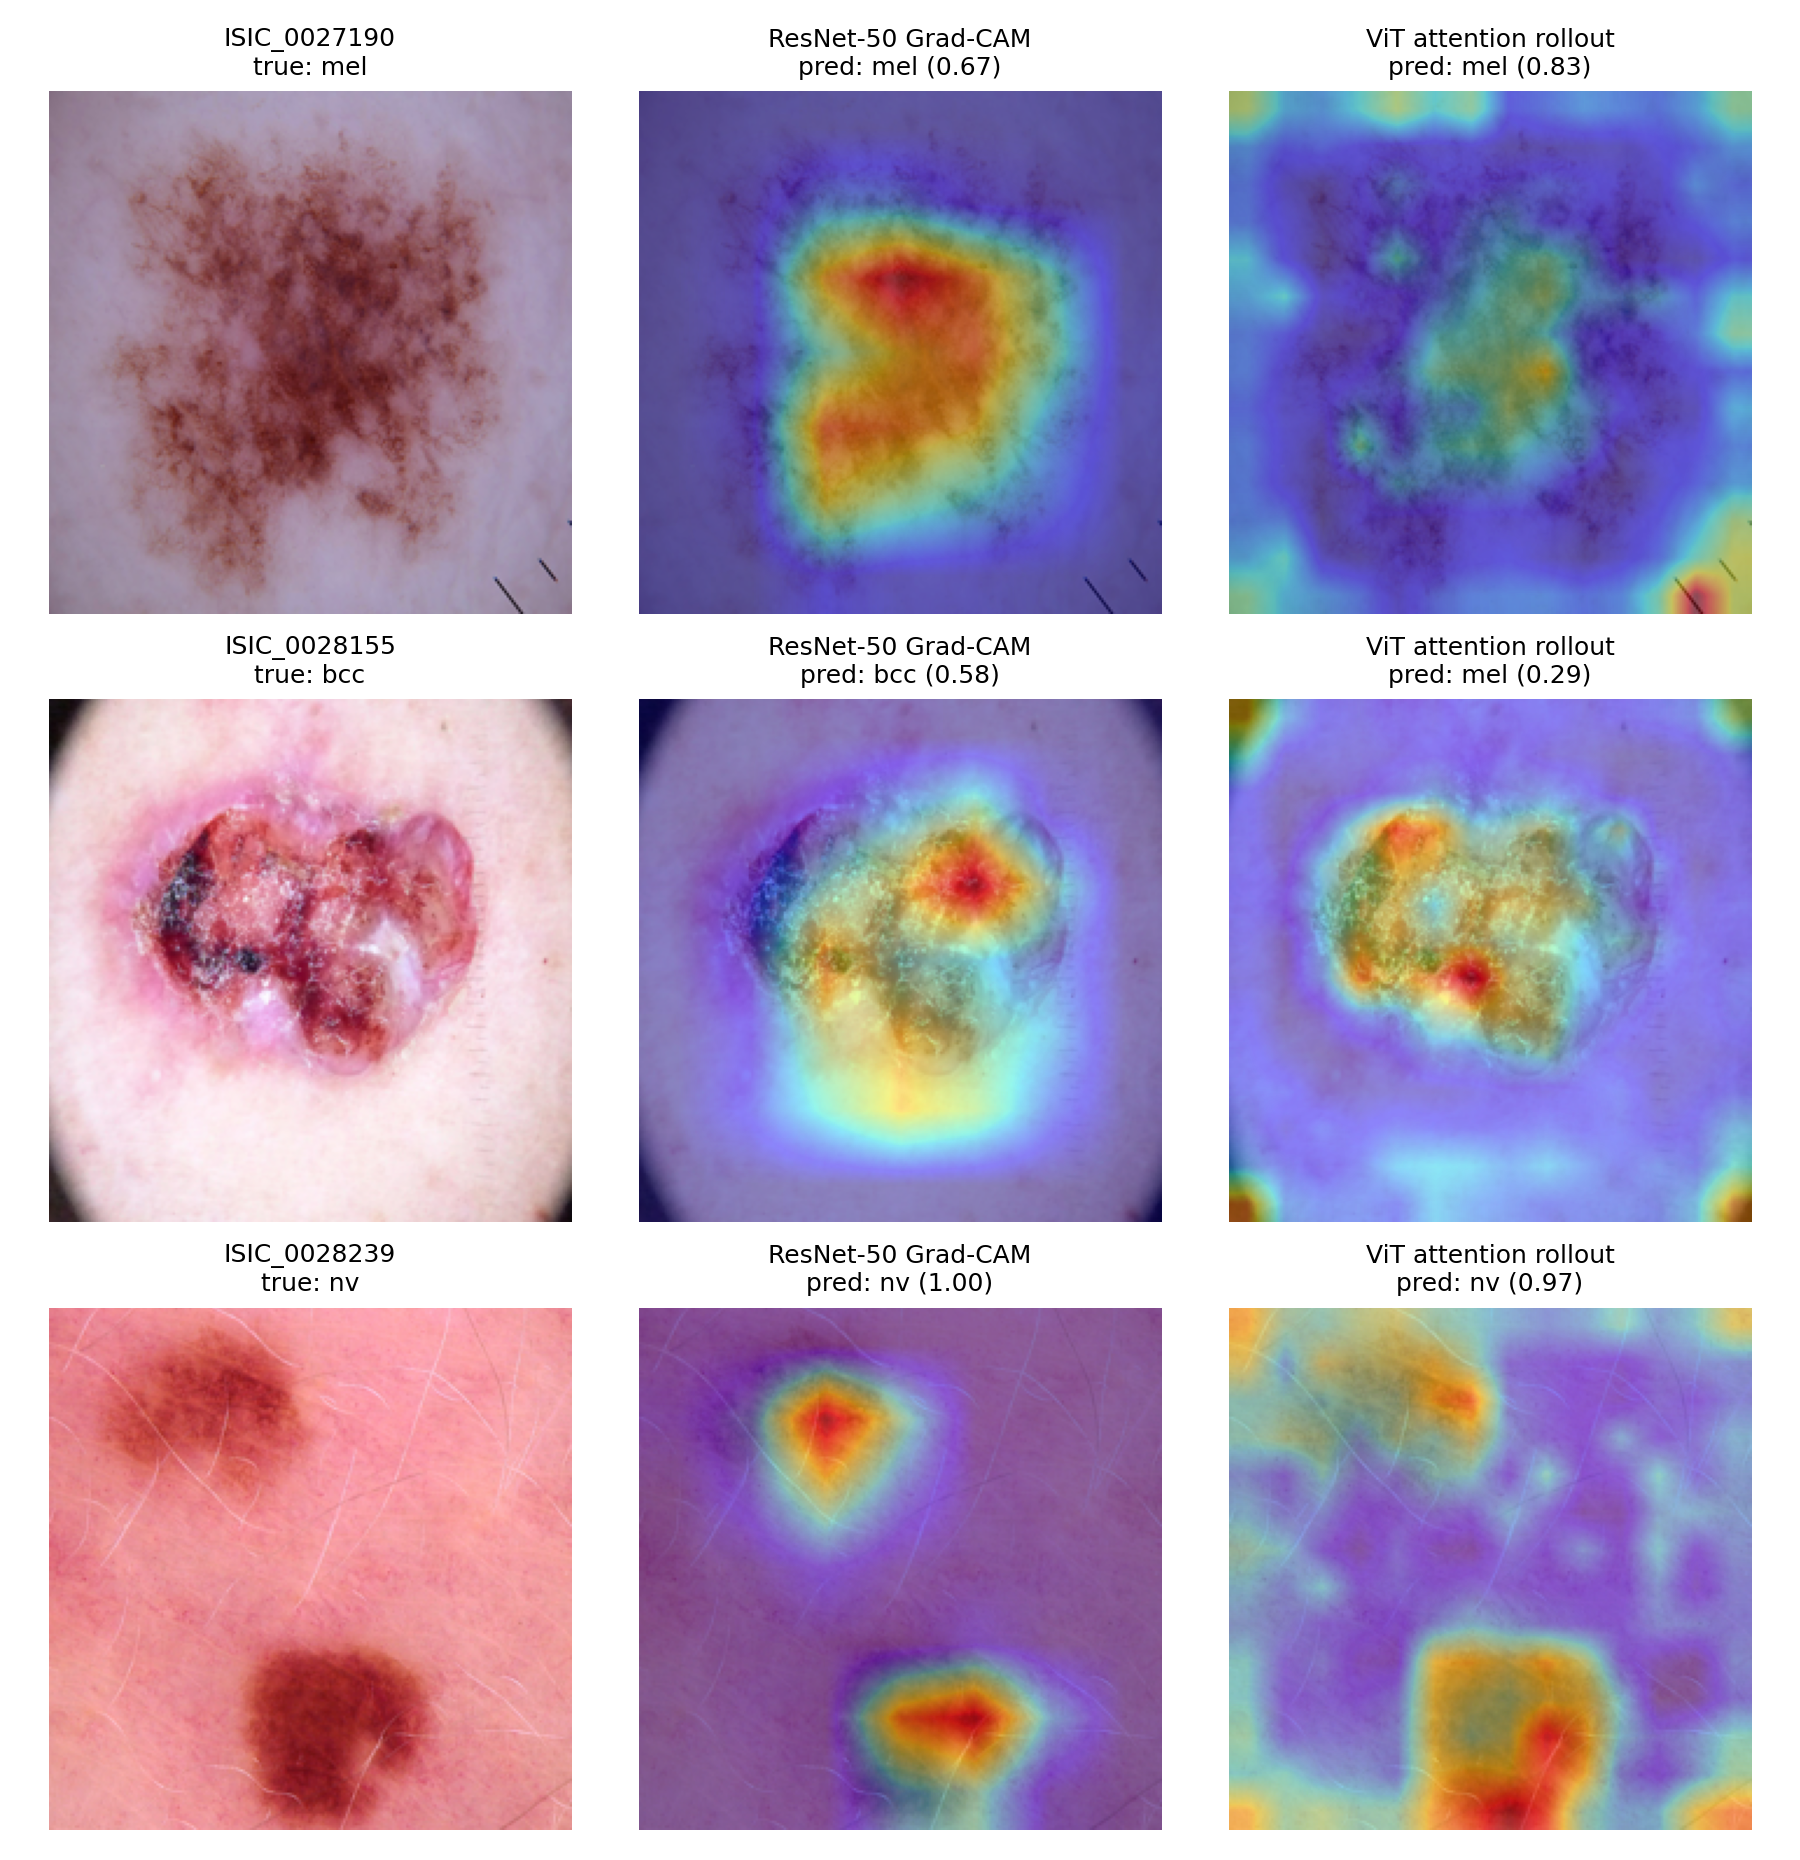
\includegraphics[width=0.62\textwidth]{supplementary/attention_map.png}}{\textit{Run scripts/visualize.py to generate this figure.}}
\caption{Left: test image with its true label. Middle: ResNet-50 Grad-CAM. Right: ViT-Base attention rollout. Titles give each model's prediction and softmax confidence.}
\label{fig:maps}
\end{figure}
